% Letter asking two department professors for feedback, BMEN 600 Group 11. Shared by both letters.
% Page 1: letter text (page1.tex). Page 2: method and models. Page 3: results.
% Numbers: run 20261113_124400 of the group repository (main, commit e1ee720), printed by export_numbers.py.
% Model details: config.json of that run and src/models.py, src/ann_to_snn.py at commit e1ee720.
% Build one letter per professor:  latexmk -pdf letter_shamsi.tex letter_kenny-lang.tex
\documentclass[10pt,letterpaper]{article}

\usepackage[letterpaper,top=0.7in,bottom=0.7in,left=0.8in,right=0.8in]{geometry}
\usepackage[T1]{fontenc}
\usepackage{mathptmx}            % Times text and maths, as in most journals
\usepackage{microtype}
\usepackage{xcolor}
\usepackage{booktabs}
\usepackage{array}
\usepackage[font=small,labelfont=bf,labelsep=period,justification=justified,singlelinecheck=false,skip=4pt]{caption}
\usepackage{tikz}
\usetikzlibrary{positioning,arrows.meta,calc,decorations.pathreplacing}
\usepackage{pgfplots}
\usepackage{pgfplotstable}
\usepackage[hidelinks]{hyperref}
\pgfplotsset{compat=1.18}

% colour-blind-safe categorical slots 1 to 3 (figure markers only)
\definecolor{snncol}{HTML}{2A78D6}
\definecolor{rsnncol}{HTML}{EB6834}
\definecolor{anncol}{HTML}{1BAF7A}
\definecolor{rangecol}{HTML}{C4CAD3}
\definecolor{boxfill}{HTML}{F3F5F8}

\setlength{\parindent}{0pt}
\setlength{\parskip}{6pt}
\pagestyle{empty}

\tikzset{
  blk/.style={draw=black!70, fill=boxfill, rounded corners=2pt, align=center, font=\footnotesize,
              minimum height=1.1cm, text width=2.32cm, inner sep=2pt},
  stage/.style={draw=black!70, fill=boxfill, rounded corners=2pt, align=center, font=\footnotesize,
               minimum height=1.6cm, text width=3.62cm, inner sep=3pt},
  arr/.style={-{Stealth[length=2.2mm]}, line width=0.6pt, color=black!70},
  lbl/.style={font=\small\bfseries, anchor=south west, inner sep=0pt},
  info/.style={font=\footnotesize\itshape, anchor=south east, inner sep=0pt, color=black!75},
}

\begin{document}
% ================================================================ PAGE 1: LETTER (input by letter_body.tex)
% \Salutation is set by the wrapper file of each professor (letter_shamsi.tex, letter_kenny-lang.tex).
16 November 2026

Dear \Salutation,

We are Lex Berezowski, Amirsaeed Ghodsinejad and Pahansith Kiriwaththuduwage, students in BMEN 600 (Group 11). We
are writing to ask for your feedback on our course project. Page 2 shows our method and the four models. Page 3 shows
our results.

\textbf{Our research question.} We want to know if a recurrent spiking neural network (RSNN) can classify four motor
imagery tasks from the electroencephalogram (EEG) better than a spiking neural network (SNN). We made the SNN by
converting EEGNet. EEGNet is a small convolutional network for EEG.

\textbf{What we did.} We used BCI Competition IV dataset 2a. It has 9 subjects and 22 EEG channels. For each subject,
we first trained every model on session 1 of five other subjects. Then we fine-tuned the model on session 1 of that
subject. We tested it on session 2 of the same subject (288 trials). We repeated this 10 times with different training
subjects, so each model has 90 test results (Figure 1). The RSNN has one recurrent layer of leaky integrate-and-fire
neurons. It has almost the same number of parameters as the converted SNN (752 and 776). We also trained a non-spiking
recurrent network (RNN) of the same size as a control. Figure 2 shows the four models.

\textbf{What we found.} These results are preliminary. The converted SNN had a mean accuracy of 0.565. The RSNN had
0.385. The SNN was better for all 9 subjects. EEGNet had 0.600. The difference
between EEGNet and the SNN was not significant ($p = 0.098$). But, in our results, the RSNN does not do better than the
converted SNN. Table 1 shows the full results of the four models, Table 2 shows the accuracy of each subject and
Table 3 shows the statistical tests.

One more model is still training. It is an RSNN with 2,560 neurons, the same number of hidden units as EEGNet.

\textbf{Our questions.} We would be grateful for your view on two points:
\begin{enumerate}\setlength{\itemsep}{2pt}\setlength{\parskip}{0pt}\setlength{\topsep}{2pt}
  \item Is our comparison fair? We matched the models by number of parameters. Should we also report the models
        matched by number of neurons?
  \item Do you see anything in our design that could explain the low accuracy of the RSNN? What would you propose to
        increase its accuracy, while keeping the comparison between the models fair?
\end{enumerate}

If you have time, we would be happy to meet for 15 to 20 minutes, in person or online. We can also send you our code
and results. Our final report is due on 4 December.

Thank you for your time.

Sincerely,\\[4pt]
Lex Berezowski, Amirsaeed Ghodsinejad and Pahansith Kiriwaththuduwage\\
BMEN 600, Group 11


% ================================================================ PAGE 2: METHOD AND MODELS
\newpage
\begin{center}
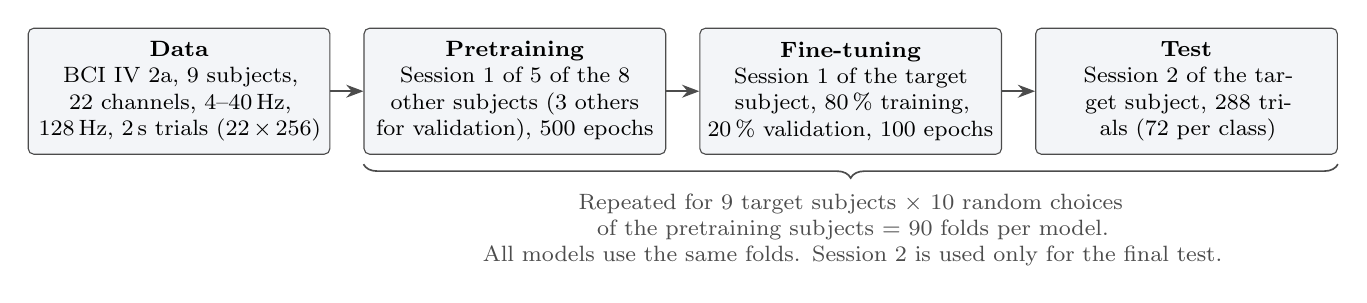
\begin{tikzpicture}[node distance=0.42cm]
  \node[stage] (d) {\textbf{Data}\\BCI IV 2a, 9 subjects, 22 channels, 4--40\,Hz, 128\,Hz, 2\,s trials (22\,$\times$\,256)};
  \node[stage, right=of d] (p) {\textbf{Pretraining}\\Session 1 of 5 of the 8 other subjects (3 others for validation), 500 epochs};
  \node[stage, right=of p] (f) {\textbf{Fine-tuning}\\Session 1 of the target subject, 80\,\% training, 20\,\% validation, 100 epochs};
  \node[stage, right=of f] (t) {\textbf{Test}\\Session 2 of the target subject, 288 trials (72 per class)};
  \draw[arr] (d) -- (p); \draw[arr] (p) -- (f); \draw[arr] (f) -- (t);
  \draw[decorate, decoration={brace, amplitude=5pt, mirror}, line width=0.6pt, color=black!70]
    ($(p.south west)+(0,-0.12)$) -- ($(t.south east)+(0,-0.12)$)
    node[midway, below=7pt, font=\footnotesize, align=center, text width=11cm]
    {Repeated for 9 target subjects $\times$ 10 random choices of the pretraining subjects = 90 folds per model.\\
     All models use the same folds. Session 2 is used only for the final test.};
\end{tikzpicture}
\captionof{figure}{Evaluation protocol. Each fold gives one test accuracy. For the statistics, the 10 repeats of a
subject are averaged, so each model has 9 paired values (one per subject).}
\end{center}

\vspace{4pt}
\begin{center}
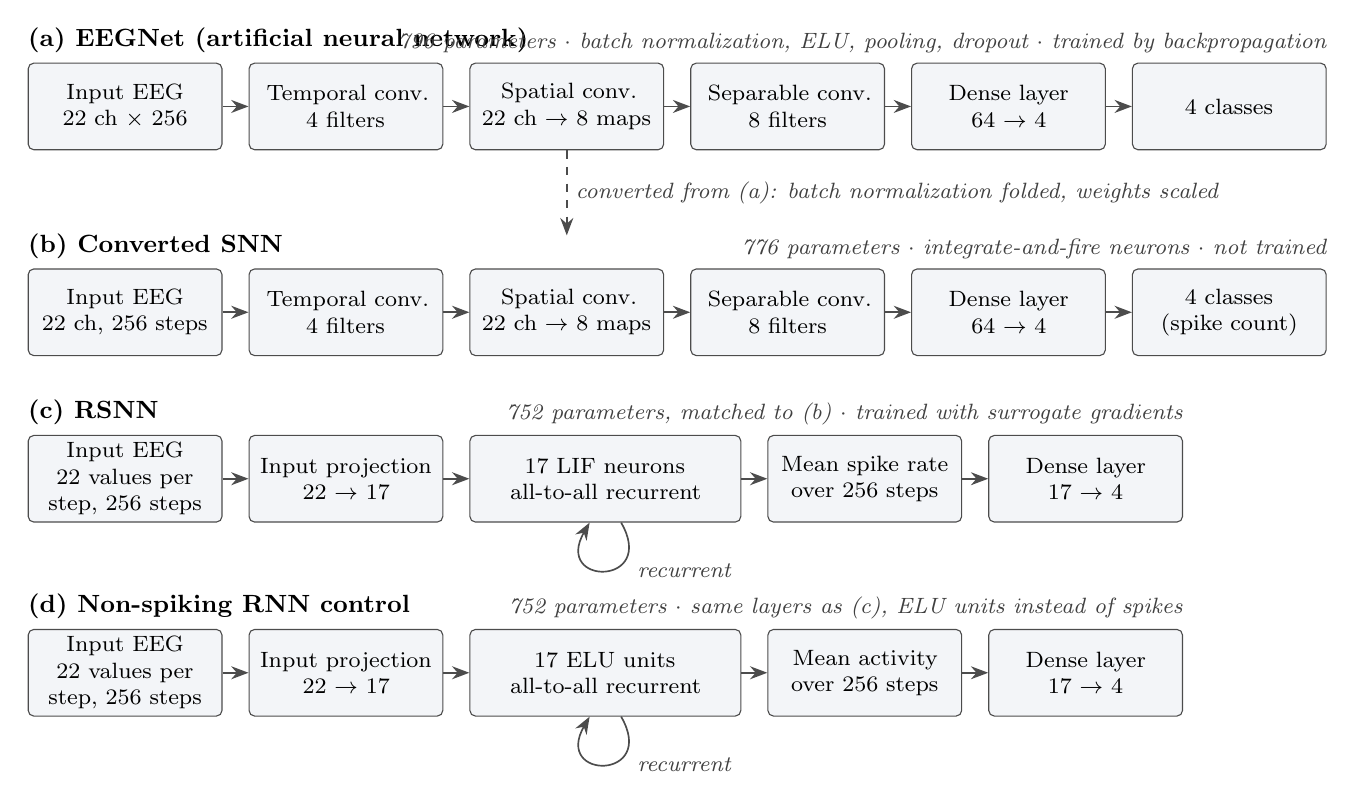
\begin{tikzpicture}[node distance=0.33cm]
  % ---- (a) EEGNet
  \node[blk] (a1) {Input EEG\\22 ch $\times$ 256};
  \node[blk, right=of a1] (a2) {Temporal conv.\\4 filters};
  \node[blk, right=of a2] (a3) {Spatial conv.\\22 ch $\to$ 8 maps};
  \node[blk, right=of a3] (a4) {Separable conv.\\8 filters};
  \node[blk, right=of a4] (a5) {Dense layer\\64 $\to$ 4};
  \node[blk, right=of a5] (a6) {4 classes};
  \foreach \i/\j in {1/2,2/3,3/4,4/5,5/6} \draw[arr] (a\i) -- (a\j);
  \node[lbl] at ($(a1.north west)+(0,0.12)$) {(a) EEGNet (artificial neural network)};
  \node[info] at ($(a6.north east)+(0,0.12)$) {796 parameters $\cdot$ batch normalization, ELU, pooling, dropout $\cdot$ trained by backpropagation};

  % ---- (b) converted SNN
  \node[blk, below=1.5cm of a1] (b1) {Input EEG\\22 ch, 256 steps};
  \node[blk, right=of b1] (b2) {Temporal conv.\\4 filters};
  \node[blk, right=of b2] (b3) {Spatial conv.\\22 ch $\to$ 8 maps};
  \node[blk, right=of b3] (b4) {Separable conv.\\8 filters};
  \node[blk, right=of b4] (b5) {Dense layer\\64 $\to$ 4};
  \node[blk, right=of b5] (b6) {4 classes\\(spike count)};
  \foreach \i/\j in {1/2,2/3,3/4,4/5,5/6} \draw[arr] (b\i) -- (b\j);
  \node[lbl] at ($(b1.north west)+(0,0.12)$) {(b) Converted SNN};
  \node[info] at ($(b6.north east)+(0,0.12)$) {776 parameters $\cdot$ integrate-and-fire neurons $\cdot$ not trained};
  \draw[arr, dashed] (a3.south) -- ($(b3.north)+(0,0.42)$) node[midway, right, font=\footnotesize\itshape,
    color=black!75, inner sep=3pt] {converted from (a): batch normalization folded, weights scaled};

  % ---- (c) RSNN
  \node[blk, below=1.0cm of b1] (c1) {Input EEG\\22 values per step, 256 steps};
  \node[blk, right=of c1] (c2) {Input projection\\22 $\to$ 17};
  \node[blk, right=of c2, text width=3.3cm, minimum height=1.1cm] (c3) {17 LIF neurons\\all-to-all recurrent};
  \node[blk, right=of c3] (c4) {Mean spike rate\\over 256 steps};
  \node[blk, right=of c4] (c5) {Dense layer\\17 $\to$ 4};
  \foreach \i/\j in {1/2,2/3,3/4,4/5} \draw[arr] (c\i) -- (c\j);
  \draw[arr] ($(c3.south)+(0.2,0)$) to[out=-60, in=-120, looseness=6] node[right=8pt, font=\footnotesize\itshape, color=black!75] {recurrent} ($(c3.south)+(-0.2,0)$);
  \node[lbl] at ($(c1.north west)+(0,0.12)$) {(c) RSNN};
  \node[info] at ($(c5.north east)+(0,0.12)$) {752 parameters, matched to (b) $\cdot$ trained with surrogate gradients};

  % ---- (d) RNN control
  \node[blk, below=1.35cm of c1] (e1) {Input EEG\\22 values per step, 256 steps};
  \node[blk, right=of e1] (e2) {Input projection\\22 $\to$ 17};
  \node[blk, right=of e2, text width=3.3cm, minimum height=1.1cm] (e3) {17 ELU units\\all-to-all recurrent};
  \node[blk, right=of e3] (e4) {Mean activity\\over 256 steps};
  \node[blk, right=of e4] (e5) {Dense layer\\17 $\to$ 4};
  \foreach \i/\j in {1/2,2/3,3/4,4/5} \draw[arr] (e\i) -- (e\j);
  \draw[arr] ($(e3.south)+(0.2,0)$) to[out=-60, in=-120, looseness=6] node[right=8pt, font=\footnotesize\itshape, color=black!75] {recurrent} ($(e3.south)+(-0.2,0)$);
  \node[lbl] at ($(e1.north west)+(0,0.12)$) {(d) Non-spiking RNN control};
  \node[info] at ($(e5.north east)+(0,0.12)$) {752 parameters $\cdot$ same layers as (c), ELU units instead of spikes};
\end{tikzpicture}
\captionof{figure}{The four compared models. Conv.: convolution. ELU: exponential linear unit. LIF: leaky
integrate-and-fire.}
\end{center}

% ================================================================ PAGE 3: RESULTS
\newpage
\captionof{table}{Performance of the four models on the test session (mean over 9 subjects; each subject's value is the
mean of its 10 repeats). SD: standard deviation across subjects. Above chance: subjects with accuracy above the binomial
threshold 0.292 (288 trials, 4 classes, $\alpha = 0.05$).}
\begin{center}\small
\begin{tabular}{@{}lrcccccc@{}}
\toprule
 & & \multicolumn{4}{c}{Accuracy} & & \\
\cmidrule(lr){3-6}
Model & Parameters & Mean $\pm$ SD & Median & Min & Max & Cohen's $\kappa$ & Macro-F1 \\
\midrule
EEGNet (a)          & 796 & 0.600 $\pm$ 0.150 & 0.628 & 0.409 & 0.781 & 0.466 $\pm$ 0.201 & 0.586 $\pm$ 0.153 \\
Converted SNN (b)   & 776 & 0.565 $\pm$ 0.154 & 0.618 & 0.366 & 0.756 & 0.420 $\pm$ 0.205 & 0.542 $\pm$ 0.166 \\
RSNN (c)            & 752 & 0.385 $\pm$ 0.100 & 0.374 & 0.275 & 0.515 & 0.180 $\pm$ 0.133 & 0.340 $\pm$ 0.095 \\
RNN control (d)     & 752 & 0.411 $\pm$ 0.106 & 0.376 & 0.275 & 0.542 & 0.215 $\pm$ 0.142 & 0.378 $\pm$ 0.110 \\
\midrule
\multicolumn{8}{@{}l}{Subjects above chance: EEGNet 9/9, converted SNN 9/9, RSNN 6/9, RNN control 7/9.} \\
\bottomrule
\end{tabular}
\end{center}

\vspace{2pt}
\captionof{table}{Test accuracy of each target subject (mean of 10 repeats). $^\dagger$ Not above the chance threshold
0.292. The best model of each subject is in bold.}
\begin{center}\small
\begin{tabular}{@{}lrrrrrrrrr@{}}
\toprule
Model & S1 & S2 & S3 & S4 & S5 & S6 & S7 & S8 & S9 \\
\midrule
EEGNet (a)        & \textbf{0.712} & \textbf{0.409} & \textbf{0.781} & \textbf{0.524} & \textbf{0.413} & \textbf{0.458} & 0.628 & \textbf{0.737} & 0.736 \\
Converted SNN (b) & 0.618 & 0.400 & 0.734 & 0.463 & 0.366 & 0.416 & \textbf{0.679} & 0.656 & \textbf{0.756} \\
RSNN (c)          & 0.453 & 0.281$^\dagger$ & 0.477 & 0.374 & 0.275$^\dagger$ & 0.284$^\dagger$ & 0.314 & 0.515 & 0.493 \\
RNN control (d)   & 0.516 & 0.275$^\dagger$ & 0.542 & 0.376 & 0.285$^\dagger$ & 0.328 & 0.371 & 0.483 & 0.523 \\
\bottomrule
\end{tabular}
\end{center}

\vspace{2pt}
\pgfplotstableread[col sep=comma]{
row,label,snn,rsnn,ann,mid,half
1,Subject 1,0.618,0.453,0.712,0.5825,0.1297
2,Subject 2,0.400,0.281,0.409,0.3453,0.0641
3,Subject 3,0.734,0.477,0.781,0.6292,0.1521
4,Subject 4,0.463,0.374,0.524,0.4489,0.0746
5,Subject 5,0.366,0.275,0.413,0.3438,0.0691
6,Subject 6,0.416,0.284,0.458,0.3712,0.0868
7,Subject 7,0.679,0.314,0.628,0.4961,0.1826
8,Subject 8,0.656,0.515,0.737,0.6257,0.1111
9,Subject 9,0.756,0.493,0.736,0.6244,0.1317
10,Mean,0.565,0.385,0.600,0.4924,0.1074
}\persubject
\begin{center}
\begin{tikzpicture}
\begin{axis}[
  width=0.92\linewidth, height=6.1cm,
  font=\footnotesize,
  xmin=0.2, xmax=0.8, ymin=0.4, ymax=10.6, y dir=reverse,
  ytick={1,...,10},
  yticklabels={Subject 1,Subject 2,Subject 3,Subject 4,Subject 5,Subject 6,Subject 7,Subject 8,Subject 9,\textbf{Mean}},
  xtick={0.2,0.3,...,0.8},
  xticklabel style={/pgf/number format/fixed,/pgf/number format/precision=1},
  xlabel={Test accuracy (session 2, 288 trials)},
  xmajorgrids, major grid style={color=black!10},
  axis line style={color=black!50}, tick style={color=black!50},
  legend style={at={(1,1.02)}, anchor=south east, draw=none, legend columns=3, font=\footnotesize,
                /tikz/every even column/.append style={column sep=8pt}},
]
  \draw[dashed, color=black!60, line width=0.7pt] (axis cs:0.2917,0.4) -- (axis cs:0.2917,10.6);
  \node[anchor=north west, font=\scriptsize, color=black!70, fill=white, inner sep=1pt] at (axis cs:0.2917,0.45) {chance 0.292};
  \draw[color=black!40] (axis cs:0.2,9.5) -- (axis cs:0.8,9.5);
  \addplot[forget plot, draw=none, mark=none,
           error bars/.cd, x dir=both, x explicit, error mark=none,
           error bar style={line width=2pt, color=rangecol}]
    table[x=mid, y=row, x error=half] {\persubject};
  \addplot[only marks, mark=*, mark size=2.6pt, mark options={fill=snncol, draw=white, line width=0.8pt}]
    table[x=snn, y=row] {\persubject};
  \addlegendentry{Converted SNN}
  \addplot[only marks, mark=*, mark size=2.6pt, mark options={fill=rsnncol, draw=white, line width=0.8pt}]
    table[x=rsnn, y=row] {\persubject};
  \addlegendentry{RSNN}
  \addplot[only marks, mark=*, mark size=2.6pt, mark options={fill=anncol, draw=white, line width=0.8pt}]
    table[x=ann, y=row] {\persubject};
  \addlegendentry{EEGNet}
\end{axis}
\end{tikzpicture}
\captionof{figure}{Test accuracy per subject for the three models of the research question (values of Table 2). The
grey bar spans the three models. The dashed line is the chance threshold.}
\end{center}

\vspace{2pt}
\captionof{table}{Paired comparisons over the 9 subjects. $\Delta$: mean difference (first model minus second model).
Exact two-sided Wilcoxon signed-rank test on the subject accuracies, Holm correction over the three planned comparisons.}
\begin{center}\small
\begin{tabular}{@{}lrrrcc@{}}
\toprule
Comparison & $\Delta$ accuracy & $\Delta$ $\kappa$ & $\Delta$ macro-F1 & First model higher & $p$ (Holm) \\
\midrule
Converted SNN $-$ RSNN (research question) & $+0.180$ & $+0.240$ & $+0.202$ & 9 of 9 & 0.012 \\
EEGNet $-$ RSNN                            & $+0.215$ & $+0.286$ & $+0.246$ & 9 of 9 & 0.012 \\
EEGNet $-$ converted SNN                   & $+0.034$ & $+0.046$ & $+0.044$ & 7 of 9 & 0.098 \\
\midrule
RNN control $-$ RSNN (effect of spiking)   & $+0.026$ & $+0.035$ & $+0.038$ & 7 of 9 & 0.074$^\ast$ \\
\bottomrule
\multicolumn{6}{@{}l}{\footnotesize $^\ast$ Not part of the planned comparisons, so not corrected. With 9 subjects, the
smallest possible Holm-corrected $p$ is 0.012.}
\end{tabular}
\end{center}

\end{document}
